\documentclass{beamer}
\mode<presentation>
{
  \usetheme{Montpellier}
%  \setbeamercovered{transparent}
  \setbeamercovered{invisible}
}
\usepackage[english]{babel}
\usepackage[latin1]{inputenc}
\usepackage{graphicx,times,tkz-graph,mathrsfs,listings,verbatim,tikz,caption,amsmath}
\usetikzlibrary{shapes.geometric}%   
\usepackage[T1]{fontenc}
\newcommand{\E}{\operatorname{E}}
\newcommand{\VE}{\operatorname{VE}}
\lstset{
	numberstyle=\footnotesize,
	basicstyle=\ttfamily\tiny}
\graphicspath{{WIgraphs/}}
%\graphicspath{{C:/Users/VOR1/Dropbox/Misc work/Waning immunity/WI project/WIgraphs/}}
%%%%%%%%%%%%%%%%%%%%%%%%%%%%%%%%%%%%%%%%%%%%%%%%%%%%%%%%%%%%%%%5
\title[Waning] % (optional, use only with long paper titles)
{``Intra-Seasonal Waning'' as Methodological Artifact}
\date{10/10/2018}
%
%
\author{Ivo M. Foppa}
% If you wish to uncover everything in a step-wise fashion, uncomment
% the following command:
%\beamerdefaultoverlayspecification{<+->}
\begin{document}
%
	\begin{frame}
	\titlepage
	\end{frame}
%
%
\section{Introduction}
\begin{frame}{Waning VE}
\footnotesize
%
\begin{itemize}
\item Since 2015, there have been numerous reports, from the US, Europe and beyond, suggesting that influenza Vaccine effectiveness (VE) declines over the season
\item \ldots
	%
\end{itemize}
\end{frame}	
%

\begin{frame}
%
Petrie JG et al., ``Modest waning of influenza vaccine efficacy and antibody titers during the 2007-2008 influenza season'', \textit{JID} 2016;214(8):
\bigskip

\centering
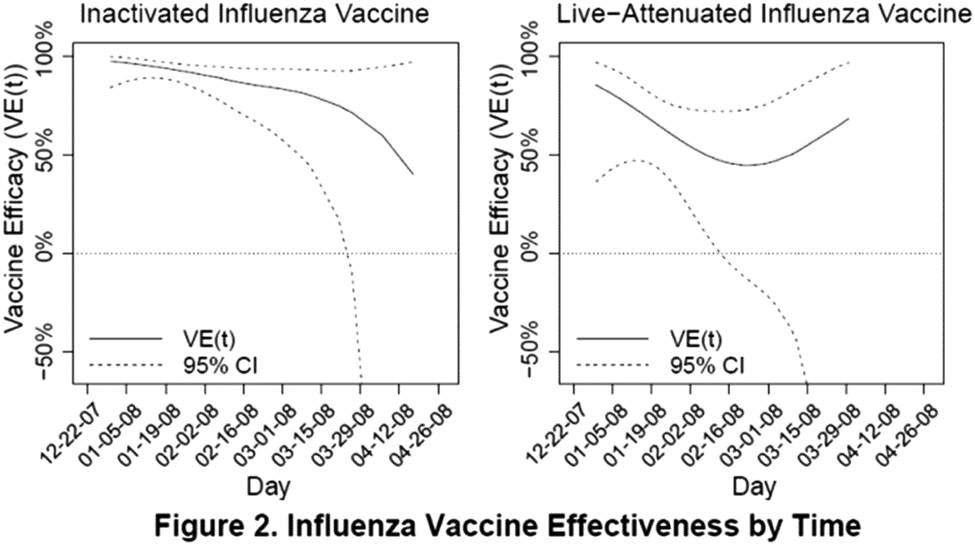
\includegraphics[width=.8\textwidth]{Petrie_waning}

\end{frame}	
%
\begin{frame}
%
Gherasim A et al., ``Waning protection of influenza vaccine against mild laboratory confirmed influenza A (H3N2) and B in Spain, season 2014-15'', \textit{Vaccine} 2016;34(20):
\bigskip

\centering
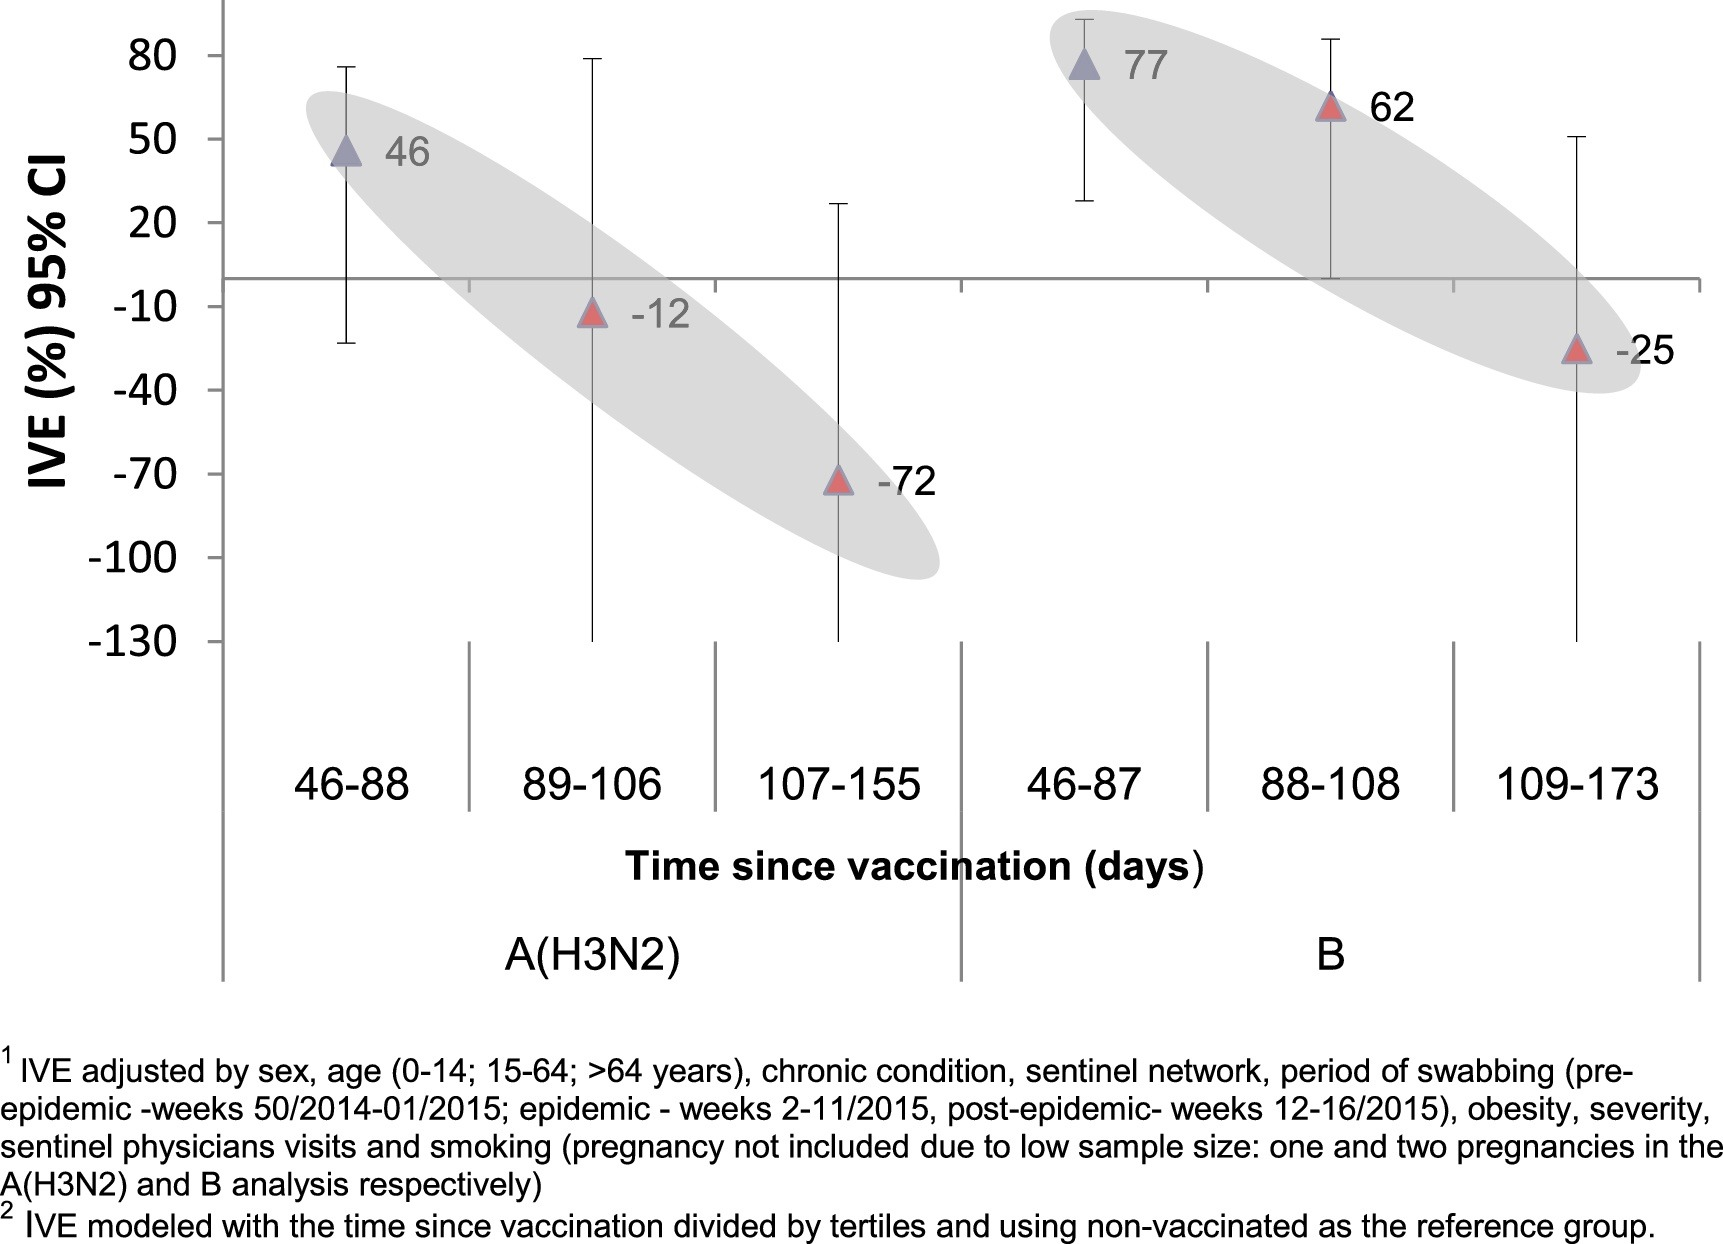
\includegraphics[width=.6\textwidth]{Spain_waning}

\end{frame}	
%
\section{Methdological sources of ``waning effect''}
\begin{frame}
Lipsitch editiorial (CID, 2018):
\begin{itemize}
	\item<2->[] ``Even if the vaccine effect does not wane over time, then such waning will nonetheless appear to occur in most studies [\ldots]'' (``leaky'' vaccines)
	\item<3->[] This will happen if:\begin{enumerate}
		\item<4-> ``there is heterogeneous risk of becoming infected within those who are vaccinated''
		\item<5-> ``some trial participants during the course of the trial become infected but are not counted as cases'' \uncover<6->{\textbf{$\leftarrow$ Not relevant to TND studies!}} 
		\item<7-> What if the vaccine is not leaky?
	\end{enumerate}
\end{itemize}
\end{frame}
\begin{frame}{Vaccine models}
\begin{itemize}
\item ``Leaky'' model: Those susceptible before vaccination have a risk of $\lambda_0 k$ of becoming infected during a contact if an unvaccinated susceptible has risk $\lambda_0$.
\end{itemize}
\end{frame}
%
%
\subsection{Approach}
\begin{frame}{Approach}
%
\begin{itemize}
	\item<2-> Simulation of seasonal influenza epidemics using simple SIR ODE models
	\item<3-> Implement two scenarios (``leaky'', ''all-or-none'' with two viruses)
	\item<4-> Use numerical solutions to ODEs to generate TND data
	\item<5-> Calculate VE ``estimates'' and true VE
\end{itemize}
\end{frame}
%
\subsection{First scenario: ``Leaky'' vaccine}
\begin{frame}
\textbf{``Leaky'' vaccine:}
The instantaneous infection risk of those vaccinated is reduced by a constant factor (e.g. difference in infectious dose):
\begin{itemize}
	\item<2-> Risk at time $t$ in those \textbf{not vaccinated}:  \[\lambda_0(t)\]
	\item<2-> Risk at time $t$ in those \textbf{vaccinated}:
	\[\lambda_1(t)=\lambda_0(t)\;\alpha; \; \alpha \in [0,1]\]
	\item<3-> $\operatorname{VE} = 1 - \frac{\lambda_1(t)}{\lambda_0(t)} = 1 - \frac{\lambda_0(t)\;\alpha}{\lambda_0(t)} = 1-\alpha$
\end{itemize}
\end{frame}
%
\begin{frame}{Deterministic transmission modeling, refresher}
\begin{itemize}
	\item<2-> Basic SIR model
		\begin{figure}[h]
\begin{center}
				\begin {tikzpicture}[>= stealth,scale=1]
\node(S)[rectangle,minimum width=.8cm,draw] at (-2,0) {S};
%
\node (I)[rectangle,minimum width=.8cm,draw] at (0,0) {I};
\node (R)[rectangle,minimum width=.8cm,draw] at (2,0) {R};
%
\draw[->](S) edge node[above] {$\beta I$} (I);
\draw[->](I) edge node[above] {$\gamma$}(R);
\end {tikzpicture}
\end{center}\end{figure}
\item<3-> {\footnotesize Differential equation representation  (Kermack\&McKendrick, 1927):
\begin{align*}
\frac{dS}{dt} &= - \beta I S\\
\frac{dI}{dt} &=  \; \beta I S\\
\frac{dR}{dt} &= - \gamma I
\end{align*}}
\item<4> System of ODEs can be solved (numerically!), makes pretty pictures ...
\end{itemize}
%
\end{frame}
%
\begin{frame}{SIR model, ``leaky'' vaccine}
\begin{figure}[h]
	\begin{center}
		\begin {tikzpicture}[>= stealth,scale=1]
		\node(Sv)[rectangle,minimum width=.8cm,draw] at (-2,0) {$S_v$};
		%
		\node (Iv)[rectangle,minimum width=.8cm,draw] at (0,0) {$I_v$};
		\node (Rv)[rectangle,minimum width=.8cm,draw] at (2,0) {$R_v$};
		%
		\draw[->](Sv) edge node[above] {$\alpha \lambda(t)$} (Iv);
		\draw[->](Iv) edge node[above] {$\gamma$}(Rv);
		
		\node(Snv)[rectangle,minimum width=.8cm,draw] at (-2,-1) {$S_{nv}$};
		%
		\node (Inv)[rectangle,minimum width=.8cm,draw] at (0,-1) {$I_{nv}$};
		\node (Rnv)[rectangle,minimum width=.8cm,draw] at (2,-1) {$R_{nv}$};
		%
		\draw[->](Snv) edge node[above] {$\lambda(t)$} (Inv);
		\draw[->](Inv) edge node[above] {$\gamma$}(Rnv);
		\end {tikzpicture}
	\end{center}
\end{figure}
where $\lambda(t)=\beta \big(I_v + I_{nv}\big)$.
\end{frame}
\begin{frame}{VE estimates for true VE=50\%}
\centering
\includegraphics<1>[width=.7\textwidth]{Leaky_VEest_50}
\includegraphics<2>[width=.7\textwidth]{Leaky_VEest_50_cases}
\end{frame}
%
\begin{frame}{\small VE estimates for range of true VEs}
\vspace{.15em}

\centering
\includegraphics<1>[width=.7\textwidth]{VEest}
\includegraphics<2>[width=.7\textwidth]{Epicurve}
\end{frame}
%
\begin{frame}{Mechanism for reduced VE over season, ``leaky'' vaccine}
\begin{itemize}
	\item True VE remains unchanged
	\item Decrease in VE due to \textbf{bias}: Faster depletion of unvaccinated susceptibles, compared to vaccinated susceptibles
\end{itemize}
\end{frame}
%
\subsection{Second scenario: ``All-or-none'', two viruses}
\begin{frame}
%
\textbf{``All-Or-None'' Vaccine, two viruses:} Vaccination fully immunizes against  virus 2; infection with either virus immunizes fully:
 
	\onslide<2->{\begin{figure}[h]
		\begin{center}
			\begin {tikzpicture}[>= stealth,scale=1]
			\node(Sv)[rectangle,minimum width=.8cm,draw] at (-2,1.5) {$S_{v}$};
			%
			\node (Iv1)[rectangle,minimum width=.8cm,draw] at (0,1.5) {$I_{v1}$};
			\node (Rv)[rectangle,minimum width=.8cm,draw] at (2,1.5) {$R_{v}$};
			%
			\draw[->](Sv) edge node[above=-1mm] {$\lambda_1(t)$} (Iv1);
			\draw[->](Iv1) edge node[above] {$\gamma$}(Rv);
			%		
			\node(Snv)[rectangle,minimum width=.8cm,draw] at (-2,0) {$S_{nv}$};
			%
			\node (Inv1)[rectangle,minimum width=.8cm,draw] at (0,0) {$I_{nv1}$};
			\node (Inv2)[rectangle,minimum width=.8cm,draw] at (0,-1.5) {$I_{nv2}$};
			\node (Rnv)[rectangle,minimum width=.8cm,draw] at (2,0) {$R_{nv}$};
			%
			\draw[->](Snv) edge node[above=-1mm] {$\lambda_1(t)$} (Inv1);
			\draw[->](Snv) edge node[right] {$\lambda_2(t)$} (Inv2);
			\draw[->](Inv1) edge node[above] {$\gamma$}(Rnv);
			\draw[->](Inv2) edge node[left] {$\gamma$}(Rnv);
			\end {tikzpicture}
		\end{center}
	\end{figure}}
	%
\onslide<3->{\footnotesize \begin{align*}
\operatorname{VE}(t) &= 1 - \frac{\lambda_{1}(t)}{\lambda_0(t)} \\
  &= 1 - \frac{\beta_1 \big(I_{v1} + I_{nv1}\big)}{\beta_1 \big(I_{v1} + I_{nv1}\big) + \beta_2 I_{nv2}} \rightarrow\text{time dependent; both viruses}
\end{align*}}
\end{frame}
%
%
\begin{frame}{\small VE estimates over season}
\vspace{.15em}
\centering
\includegraphics<1>[width=.7\textwidth]{two_viruses1}
\includegraphics<2>[width=.7\textwidth]{two_viruses2}
\includegraphics<3>[width=.7\textwidth]{two_viruses3}
\end{frame}
	%
%
\begin{frame}{Mechanisms for reduced VE over season, ``all-or-none'' vaccine, two viruses}
\begin{itemize}
	\item \textbf{True decrease} in VE due to evolutionary process, without any decay in individual vaccine protection: Relative distribution of two viruses changes (virus 1 outcompeting virus 2)
	\item Decrease in VE due to \textbf{bias}: Faster depletion of unvaccinated susceptibles, compared to vaccinated susceptibles.
%
\end{itemize}
\end{frame}
%
%
\begin{frame}{\small Evolutionary process: Viruse 1 outcompeting virus 2}
\begin{center}
		\begin{figure}
			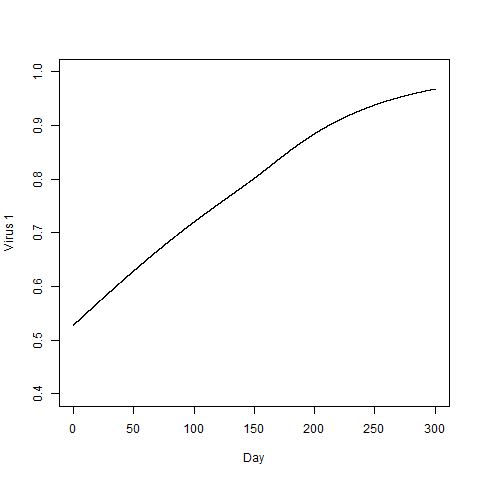
\includegraphics[width=.65\textwidth]{prop_virus1}
		\end{figure}
\end{center}
\end{frame}
%
\section{Possible solutions}
\begin{frame}{Outlook: How to deal with these issues?}
\centering
\includegraphics<2>[width=.6\textwidth]{blog-stay_tuned}
\end{frame}
\end{document}
